\section{Ex2.05 Plotting Normal Distribution}\label{sec:NormalDistribution}

\subsection{Testo esercizio}
La funzione $f(x;\mu;\sigma)$ nota come distribuzione normale o gaussiana è 
data come 
$$f(x,\mu,\sigma) = \frac{1}{{\sigma\sqrt{2\pi}}}
e^{{{-\left({x-\mu}\right)^2}/{2\sigma^2}}}$$    
dove $\mu$ è la media e $\sigma$ è la deviazione standard.

\begin{itemize}
    \item[a)] Creare una funzione $normalDistribuition(x,mu,sigma)$ che 
    restituisce il valore di $f(x,\mu,\sigma)$.
    
    \item[b)] Usa questa funzione per tracciare la gaussiana per $-5<x<5$ con 
    $\mu=0$ e $\sigma=1$.
    
    \item[c)] Usa questa funzione per tracciare le gaussiane per $-5<x<5$ con 
    $\mu=0$ e $\sigma=2$ e $0.5$ nelle stesso diagramma.
    
    \item[d)] Usa questa funzione per tracciare le gaussiane per $-5<x<5$ con 
    $\sigma=1$ e $\mu=0$, $1$, $2$ in 3 diagrammi nelle stessa figura.
\end{itemize}
\subsection{Svolgimento}
L'esercizio \'e stato semplice. Inizialmente avevo inserito $\rho=7500$ 
direttamente dentro la funzione, successivamente ho reputato opportuno inserire 
il dato via argomenti per rendere la funzione utile per qualsiasi tipo di sfera.

\subsection{Codice esercizio}
\lstinputlisting[caption = {\nameref{fnc:NormalDistribution}},
linerange = {33-40}]
{cap/Elementary/src/function/normalDistribuition.m}
\pagebreak

\subsection{Grafici con codici}
\lstinputlisting[title = {Script Ex2.05-b},
linerange = {3-10}]
{cap/Elementary/src/script/script205b.m}
\begin{figure}[h]
    \centering
    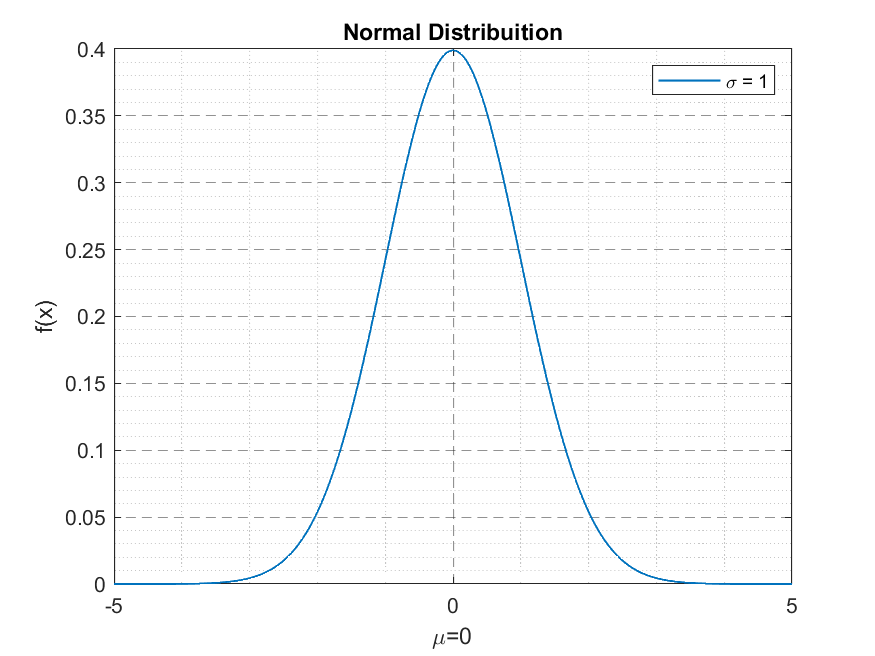
\includegraphics{cap/Elementary/img/script205b}
    \label{fig:script205b}
\end{figure}
\pagebreak

\lstinputlisting[title = {Script Ex2.05-c},
linerange = {33-40}]
{cap/Elementary/src/script/script205c.m}
\begin{figure}[h]
    \centering
    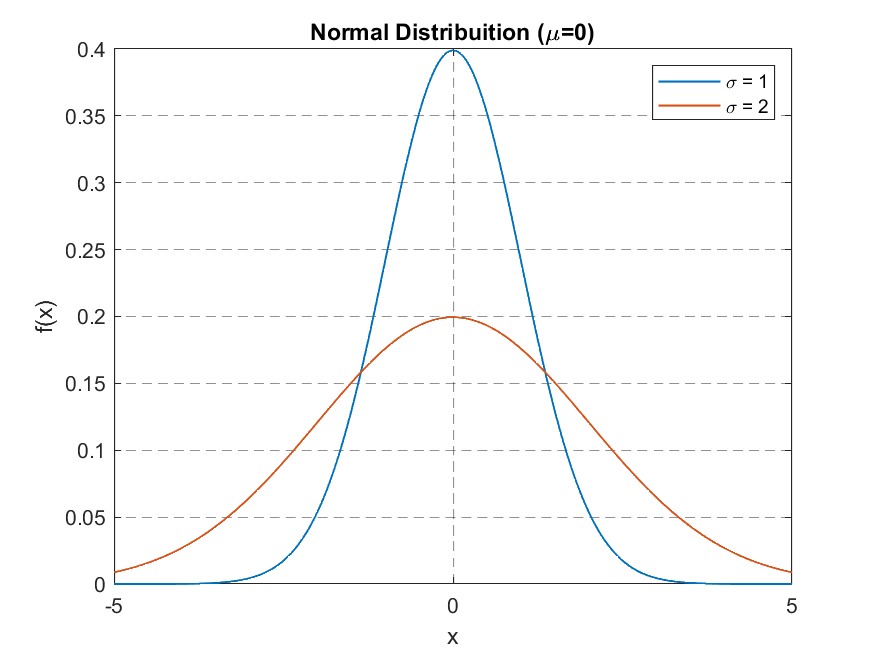
\includegraphics{cap/Elementary/img/script205c}
    \label{fig:plotscript205c}
\end{figure}
\pagebreak

\lstinputlisting[title = {Script Ex2.05-d},%
linerange ={3-17}]
{cap/Elementary/src/script/script205d.m}
\begin{figure}[h]
    \centering
    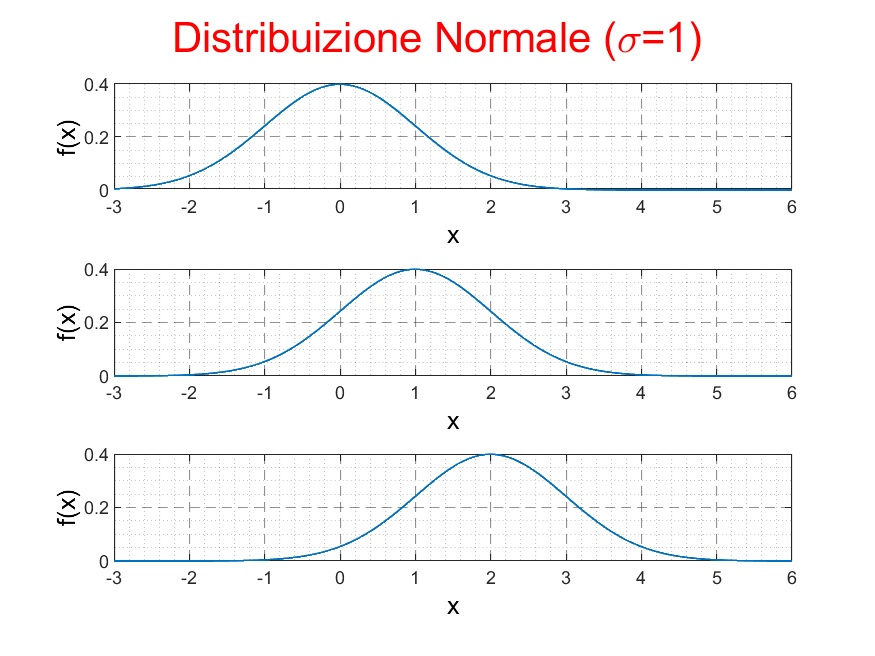
\includegraphics{cap/Elementary/img/script205d}
    \label{fig:plotscript205d}
\end{figure}